\documentclass[border=6pt]{standalone}
\usepackage{tikz}
\usepackage{amsmath,amssymb}
\usetikzlibrary{arrows.meta,shapes.geometric}

\definecolor{steelblue}{RGB}{51,115,199}
\definecolor{amber}{RGB}{217,140,26}
\definecolor{teal}{RGB}{26,166,89}
\definecolor{coral}{RGB}{217,38,38}
\definecolor{darktext}{RGB}{30,30,30}
\definecolor{midgray}{RGB}{130,130,130}
\definecolor{lightgray}{RGB}{235,235,235}
\definecolor{panelbg}{RGB}{244,244,244}

\begin{document}
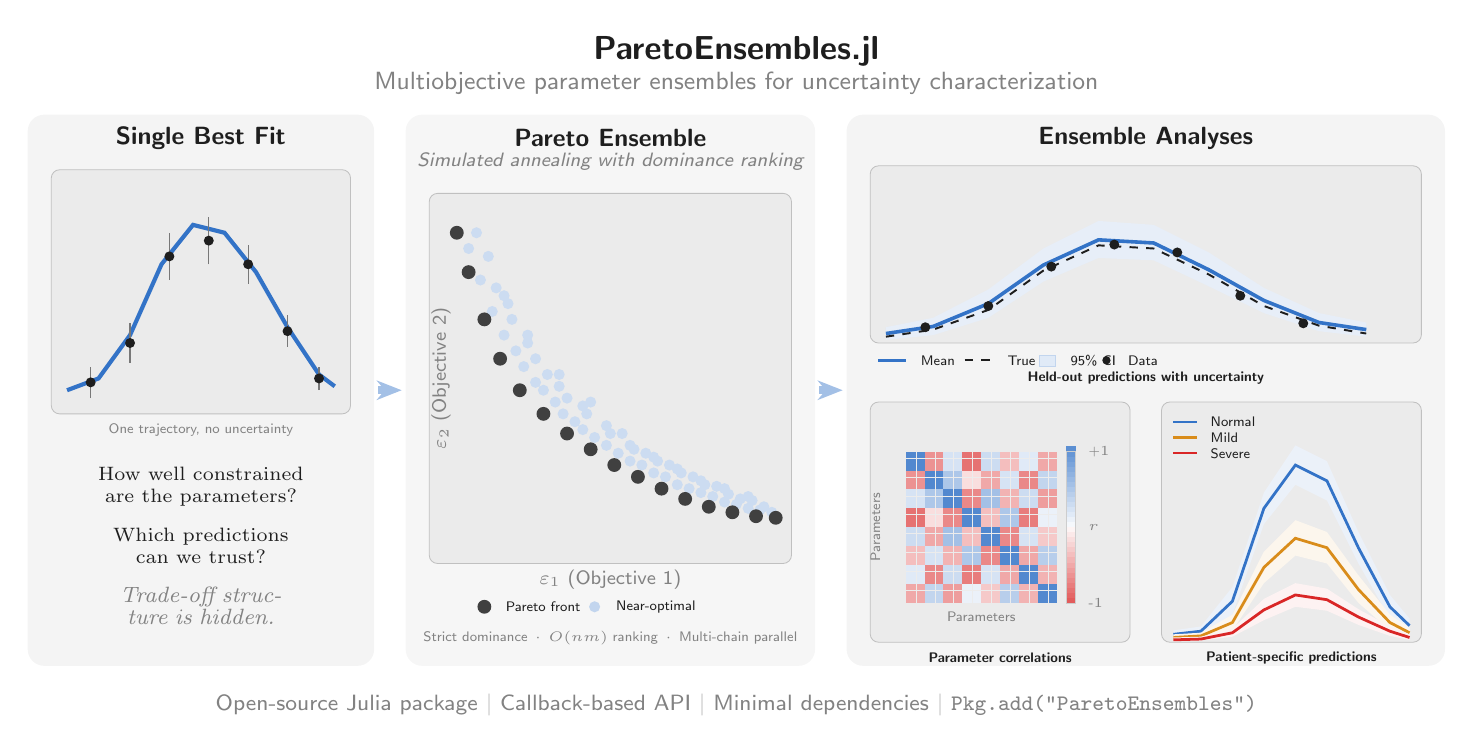
\begin{tikzpicture}[>=Stealth, every node/.style={font=\sffamily}]

% Panel backgrounds
\fill[panelbg, rounded corners=6pt] (0, 0) rectangle (4.4, 7.0);
\fill[panelbg!85!white, rounded corners=6pt] (4.8, 0) rectangle (10.0, 7.0);
\fill[panelbg, rounded corners=6pt] (10.4, 0) rectangle (18.0, 7.0);

% ════════════════════════════════════════════
% TOP TITLE
% ════════════════════════════════════════════
\node[font=\sffamily\large\bfseries, text=darktext] at (9.0, 7.8) {ParetoEnsembles.jl};
\node[font=\sffamily\small, text=midgray] at (9.0, 7.4) {%
    Multiobjective parameter ensembles for uncertainty characterization%
};

% ════════════════════════════════════════════
% LEFT: Single Best Fit
% ════════════════════════════════════════════
\node[font=\sffamily\bfseries\small, text=darktext] at (2.2, 6.7) {Single Best Fit};

\fill[lightgray, rounded corners=3pt] (0.3, 3.2) rectangle (4.1, 6.3);
\draw[midgray!50, line width=0.3pt, rounded corners=3pt] (0.3, 3.2) rectangle (4.1, 6.3);
\begin{scope}[shift={(0.3, 3.2)}, clip]
    \clip (0,0) rectangle (3.8, 3.1);
    \draw[steelblue, line width=1.5pt]
        (0.2,0.3) -- (0.6,0.45) -- (1.0,1.0) -- (1.4,1.9) -- (1.8,2.4) -- (2.2,2.3) -- (2.6,1.8) -- (3.0,1.1) -- (3.4,0.5) -- (3.6,0.35);
    \foreach \x/\y/\e in {0.5/0.4/0.2, 1.0/0.9/0.25, 1.5/2.0/0.3, 2.0/2.2/0.3, 2.5/1.9/0.25, 3.0/1.05/0.2, 3.4/0.45/0.15} {
        \draw[darktext!60, line width=0.4pt] (\x, {\y-\e}) -- (\x, {\y+\e});
        \fill[darktext] (\x, \y) circle (1.8pt);
    }
\end{scope}
\node[font=\sffamily\tiny, text=midgray] at (2.2, 3.0) {One trajectory, no uncertainty};

\node[anchor=north, text width=3.8cm, align=center, font=\scriptsize, text=darktext]
    at (2.2, 2.65) {%
    How well constrained\\are the parameters?\\[6pt]
    Which predictions\\can we trust?\\[6pt]
    {\footnotesize\itshape\color{midgray} Trade-off structure is hidden.}
};

% ════════════════════════════════════════════
% CENTER: Pareto Ensemble
% ════════════════════════════════════════════
\node[font=\sffamily\bfseries\small, text=darktext] at (7.4, 6.7) {Pareto Ensemble};
\node[font=\sffamily\scriptsize\itshape, text=midgray] at (7.4, 6.4) {Simulated annealing with dominance ranking};

\fill[lightgray, rounded corners=3pt] (5.1, 1.3) rectangle (9.7, 6.0);
\draw[midgray!50, line width=0.3pt, rounded corners=3pt] (5.1, 1.3) rectangle (9.7, 6.0);

\begin{scope}[shift={(5.1, 1.3)}, clip]
    \clip (0,0) rectangle (4.6, 4.7);
    % Near-optimal cloud
    \foreach \x/\y in {
        0.5/4.0, 0.65/3.6, 0.8/3.2, 0.85/3.5, 0.95/2.9, 1.0/3.3,
        1.1/2.7, 1.2/2.5, 1.25/2.8, 1.35/2.3, 1.45/2.2, 1.5/2.4,
        1.6/2.05, 1.7/1.9, 1.75/2.1, 1.85/1.8, 1.95/1.7, 2.0/1.9,
        2.1/1.6, 2.25/1.5, 2.3/1.65, 2.4/1.4, 2.55/1.3, 2.6/1.45,
        2.7/1.25, 2.85/1.15, 2.9/1.3, 3.0/1.1, 3.15/1.0, 3.2/1.15,
        3.3/0.95, 3.45/0.9, 3.5/1.0, 3.6/0.85, 3.75/0.78, 3.8/0.88,
        3.9/0.75, 4.05/0.7, 4.1/0.8, 4.2/0.68, 4.35/0.65,
        0.75/3.9, 1.05/3.1, 1.35/2.6, 1.65/2.25, 1.95/2.0, 2.25/1.75,
        2.55/1.5, 2.85/1.35, 3.15/1.2, 3.45/1.05, 3.75/0.95, 4.05/0.85,
        0.6/4.2, 0.95/3.4, 1.25/2.9, 1.65/2.4, 2.05/2.05, 2.45/1.65,
        2.75/1.4, 3.05/1.25, 3.35/1.1, 3.65/0.98, 3.95/0.82, 4.25/0.72
    } {
        \fill[steelblue!25] (\x, \y) circle (2pt);
    }
    % Front
    \foreach \x/\y in {
        0.35/4.2, 0.5/3.7, 0.7/3.1, 0.9/2.6, 1.15/2.2, 1.45/1.9,
        1.75/1.65, 2.05/1.45, 2.35/1.25, 2.65/1.1, 2.95/0.95, 3.25/0.82,
        3.55/0.72, 3.85/0.65, 4.15/0.6, 4.4/0.58
    } {
        \fill[darktext!85] (\x, \y) circle (2.5pt);
    }
\end{scope}
% Axis labels (inside panel)
\node[font=\sffamily\scriptsize, text=midgray] at (7.4, 1.1) {$\varepsilon_1$ (Objective 1)};
\node[font=\sffamily\scriptsize, text=midgray, rotate=90] at (5.25, 3.65) {$\varepsilon_2$ (Objective 2)};
% Legend
\fill[darktext!85] (5.8, 0.75) circle (2.5pt);
\node[font=\sffamily\tiny, text=darktext, anchor=west] at (5.95, 0.75) {Pareto front};
\fill[steelblue!30] (7.2, 0.75) circle (2pt);
\node[font=\sffamily\tiny, text=darktext, anchor=west] at (7.35, 0.75) {Near-optimal};
% Features
\node[font=\sffamily\tiny, text=midgray] at (7.4, 0.35) {%
    Strict dominance\enspace$\cdot$\enspace
    $O(nm)$ ranking\enspace$\cdot$\enspace
    Multi-chain parallel%
};

% ════════════════════════════════════════════
% RIGHT: Ensemble Analyses
% ════════════════════════════════════════════
\node[font=\sffamily\bfseries\small, text=darktext] at (14.2, 6.7) {Ensemble Analyses};

% ── Top: Held-out predictions ──
\fill[lightgray, rounded corners=3pt] (10.7, 4.1) rectangle (17.7, 6.35);
\draw[midgray!50, line width=0.3pt, rounded corners=3pt] (10.7, 4.1) rectangle (17.7, 6.35);
\begin{scope}[shift={(10.7, 4.1)}, clip]
    \clip (0,0) rectangle (7.0, 2.25);
    % Faint ensemble trajectories
    \foreach \yoff in {-0.1, -0.05, 0, 0.05, 0.1, -0.07, 0.07, -0.03, 0.03} {
        \draw[steelblue!15, line width=0.5pt]
            (0.2,{0.15+\yoff*0.4}) -- (0.8,{0.25+\yoff*0.5}) -- (1.5,{0.55+\yoff*0.8}) -- (2.2,{1.05+\yoff*1.0}) -- (2.9,{1.4+\yoff*1.0}) -- (3.6,{1.35+\yoff*0.9}) -- (4.3,{1.0+\yoff*0.7}) -- (5.0,{0.6+\yoff*0.5}) -- (5.7,{0.3+\yoff*0.3}) -- (6.3,{0.2+\yoff*0.2});
    }
    % CI band
    \fill[steelblue!12]
        (0.2,0.2) -- (0.8,0.32) -- (1.5,0.68) -- (2.2,1.2) -- (2.9,1.55) -- (3.6,1.5) -- (4.3,1.15) -- (5.0,0.7) -- (5.7,0.38) -- (6.3,0.26)
        -- (6.3,0.08) -- (5.7,0.15) -- (5.0,0.38) -- (4.3,0.72) -- (3.6,1.05) -- (2.9,1.08) -- (2.2,0.78) -- (1.5,0.32) -- (0.8,0.1) -- (0.2,0.04) -- cycle;
    % Mean
    \draw[steelblue, line width=1.3pt]
        (0.2,0.12) -- (0.8,0.21) -- (1.5,0.5) -- (2.2,0.99) -- (2.9,1.31) -- (3.6,1.27) -- (4.3,0.93) -- (5.0,0.54) -- (5.7,0.26) -- (6.3,0.17);
    % True
    \draw[darktext, line width=0.7pt, dashed]
        (0.2,0.08) -- (0.8,0.17) -- (1.5,0.42) -- (2.2,0.92) -- (2.9,1.24) -- (3.6,1.2) -- (4.3,0.87) -- (5.0,0.47) -- (5.7,0.22) -- (6.3,0.12);
    % Data
    \foreach \x/\y in {0.7/0.2, 1.5/0.47, 2.3/0.97, 3.1/1.25, 3.9/1.15, 4.7/0.6, 5.5/0.25} {
        \fill[darktext] (\x, \y) circle (1.8pt);
    }
\end{scope}
% Legend below predictions (two lines: legend then bold title)
\draw[steelblue, line width=1pt] (10.8, 3.88) -- ++(0.35, 0);
\node[font=\sffamily\tiny, text=darktext, anchor=west] at (11.22, 3.88) {Mean};
\draw[darktext, line width=0.6pt, dashed] (11.9, 3.88) -- ++(0.35, 0);
\node[font=\sffamily\tiny, text=darktext, anchor=west] at (12.32, 3.88) {True};
\fill[steelblue!15] (12.85, 3.81) rectangle ++(0.2, 0.14);
\draw[steelblue!30, line width=0.2pt] (12.85, 3.81) rectangle ++(0.2, 0.14);
\node[font=\sffamily\tiny, text=darktext, anchor=west] at (13.12, 3.88) {95\% CI};
\fill[darktext] (13.7, 3.88) circle (1.5pt);
\node[font=\sffamily\tiny, text=darktext, anchor=west] at (13.85, 3.88) {Data};
\node[font=\sffamily\tiny\bfseries, text=darktext] at (14.2, 3.65) {Held-out predictions with uncertainty};

% ── Bottom-left: Correlation heatmap ──
\fill[lightgray, rounded corners=3pt] (10.7, 0.3) rectangle (14.0, 3.35);
\draw[midgray!50, line width=0.3pt, rounded corners=3pt] (10.7, 0.3) rectangle (14.0, 3.35);
% SYMMETRIC 8×8 correlation heatmap
\def\cs{0.24}
\pgfmathsetmacro{\hmox}{10.7 + 0.45}
\pgfmathsetmacro{\hmoy}{0.3 + 0.5}
% Define upper triangle + diagonal; mirror for lower triangle
% Diagonal: all steelblue!85
% Upper triangle values (i < j mapped to row j, col i):
\foreach \i/\j/\c in {
    0/7/steelblue!85, 1/7/coral!50,    2/7/steelblue!20, 3/7/coral!65,    4/7/steelblue!25, 5/7/coral!30, 6/7/steelblue!15, 7/7/coral!40,
    0/6/coral!50,     1/6/steelblue!85, 2/6/steelblue!40, 3/6/coral!15,    4/6/coral!40,     5/6/steelblue!20, 6/6/coral!55, 7/6/steelblue!30,
    0/5/steelblue!20, 1/5/steelblue!40, 2/5/steelblue!85, 3/5/coral!55,    4/5/steelblue!45, 5/5/coral!35, 6/5/steelblue!25, 7/5/coral!45,
    0/4/coral!65,     1/4/coral!15,     2/4/coral!55,     3/4/steelblue!85, 4/4/coral!30,     5/4/steelblue!40, 6/4/coral!60, 7/4/steelblue!10,
    0/3/steelblue!25, 1/3/coral!40,     2/3/steelblue!45, 3/3/coral!30,    4/3/steelblue!85, 5/3/coral!55, 6/3/steelblue!20, 7/3/coral!25,
    0/2/coral!30,     1/2/steelblue!20, 2/2/coral!35,     3/2/steelblue!40, 4/2/coral!55,    5/2/steelblue!85, 6/2/coral!40, 7/2/steelblue!35,
    0/1/steelblue!15, 1/1/coral!55,     2/1/steelblue!25, 3/1/coral!60,    4/1/steelblue!20, 5/1/coral!40, 6/1/steelblue!85, 7/1/coral!35,
    0/0/coral!40,     1/0/steelblue!30, 2/0/coral!45,     3/0/steelblue!10, 4/0/coral!25,    5/0/steelblue!35, 6/0/coral!35, 7/0/steelblue!85
} {
    \fill[\c] ({\i*\cs+\hmox}, {\j*\cs+\hmoy}) rectangle +({\cs}, {\cs});
}
\draw[midgray!15, line width=0.15pt, step=\cs]
    (\hmox, \hmoy) grid ({8*\cs+\hmox},{8*\cs+\hmoy});
% Axis labels
\node[font=\sffamily\tiny, text=midgray, rotate=90, anchor=south]
    at ({\hmox - 0.2}, {\hmoy + 4*\cs}) {Parameters};
\node[font=\sffamily\tiny, text=midgray]
    at ({\hmox + 4*\cs}, {\hmoy - 0.17}) {Parameters};
% Color bar
\pgfmathsetmacro{\cbx}{8*\cs + \hmox + 0.12}
\pgfmathsetmacro{\cbh}{8*\cs}
\foreach \k in {0,...,30} {
    \pgfmathsetmacro{\yy}{\hmoy + \k*\cbh/30}
    \ifnum\k<15
        \fill[coral!\the\numexpr 75 - \k*5\relax] (\cbx, \yy) rectangle ++(0.12, {\cbh/30 + 0.003});
    \else
        \fill[steelblue!\the\numexpr (\k-15)*5 + 5\relax] (\cbx, \yy) rectangle ++(0.12, {\cbh/30 + 0.003});
    \fi
}
\draw[midgray!40, line width=0.2pt] (\cbx, \hmoy) rectangle ++(0.12, \cbh);
\node[font=\sffamily\tiny, text=midgray, anchor=west] at ({\cbx + 0.16}, \hmoy) {$\text{-}1$};
\node[font=\sffamily\tiny, text=midgray, anchor=west] at ({\cbx + 0.16}, {\hmoy + \cbh/2}) {$r$};
\node[font=\sffamily\tiny, text=midgray, anchor=west] at ({\cbx + 0.16}, {\hmoy + \cbh}) {$\text{+}1$};
% Title
\node[font=\sffamily\tiny\bfseries, text=darktext] at (12.35, 0.1) {Parameter correlations};

% ── Bottom-right: Patient-specific predictions ──
\fill[lightgray, rounded corners=3pt] (14.4, 0.3) rectangle (17.7, 3.35);
\draw[midgray!50, line width=0.3pt, rounded corners=3pt] (14.4, 0.3) rectangle (17.7, 3.35);
\begin{scope}[shift={(14.4, 0.3)}, clip]
    \clip (0,0) rectangle (3.3, 3.05);
    % Normal
    \fill[steelblue!10]
        (0.15,0.15) -- (0.5,0.2) -- (0.9,0.7) -- (1.3,1.9) -- (1.7,2.5) -- (2.1,2.3) -- (2.5,1.4) -- (2.9,0.6) -- (3.15,0.3)
        -- (3.15,0.12) -- (2.9,0.3) -- (2.5,1.0) -- (2.1,1.8) -- (1.7,2.0) -- (1.3,1.5) -- (0.9,0.35) -- (0.5,0.08) -- (0.15,0.05) -- cycle;
    \draw[steelblue, line width=1pt]
        (0.15,0.1) -- (0.5,0.14) -- (0.9,0.52) -- (1.3,1.7) -- (1.7,2.25) -- (2.1,2.05) -- (2.5,1.2) -- (2.9,0.45) -- (3.15,0.21);
    % Mild
    \fill[amber!8]
        (0.15,0.1) -- (0.5,0.12) -- (0.9,0.35) -- (1.3,1.15) -- (1.7,1.55) -- (2.1,1.4) -- (2.5,0.85) -- (2.9,0.35) -- (3.15,0.18)
        -- (3.15,0.07) -- (2.9,0.15) -- (2.5,0.5) -- (2.1,1.0) -- (1.7,1.1) -- (1.3,0.75) -- (0.9,0.15) -- (0.5,0.05) -- (0.15,0.03) -- cycle;
    \draw[amber, line width=1pt]
        (0.15,0.06) -- (0.5,0.08) -- (0.9,0.25) -- (1.3,0.95) -- (1.7,1.32) -- (2.1,1.2) -- (2.5,0.67) -- (2.9,0.25) -- (3.15,0.12);
    % Severe
    \fill[coral!6]
        (0.15,0.06) -- (0.5,0.07) -- (0.9,0.17) -- (1.3,0.55) -- (1.7,0.75) -- (2.1,0.68) -- (2.5,0.42) -- (2.9,0.2) -- (3.15,0.1)
        -- (3.15,0.03) -- (2.9,0.08) -- (2.5,0.22) -- (2.1,0.4) -- (1.7,0.45) -- (1.3,0.28) -- (0.9,0.07) -- (0.5,0.02) -- (0.15,0.01) -- cycle;
    \draw[coral, line width=1pt]
        (0.15,0.03) -- (0.5,0.04) -- (0.9,0.12) -- (1.3,0.41) -- (1.7,0.6) -- (2.1,0.54) -- (2.5,0.32) -- (2.9,0.14) -- (3.15,0.06);
\end{scope}
% Legend
\draw[steelblue, line width=0.8pt] (14.55, 3.1) -- ++(0.3, 0);
\node[font=\sffamily\tiny, text=darktext, anchor=west] at (14.9, 3.1) {Normal};
\draw[amber, line width=0.8pt] (14.55, 2.9) -- ++(0.3, 0);
\node[font=\sffamily\tiny, text=darktext, anchor=west] at (14.9, 2.9) {Mild};
\draw[coral, line width=0.8pt] (14.55, 2.7) -- ++(0.3, 0);
\node[font=\sffamily\tiny, text=darktext, anchor=west] at (14.9, 2.7) {Severe};
% Title
\node[font=\sffamily\tiny\bfseries, text=darktext] at (16.05, 0.1) {Patient-specific predictions};

% ════════════════════════════════════════════
% ARROWS (span the full gap between panels)
% ════════════════════════════════════════════
\draw[-{Stealth[length=9pt,width=7pt]}, line width=3pt, color=steelblue!45]
    (4.45, 3.5) -- (4.75, 3.5);
\draw[-{Stealth[length=9pt,width=7pt]}, line width=3pt, color=steelblue!45]
    (10.05, 3.5) -- (10.35, 3.5);

% ════════════════════════════════════════════
% Bottom tagline
% ════════════════════════════════════════════
\node[font=\sffamily\footnotesize, text=midgray] at (9.0, -0.5) {
    Open-source Julia package \textcolor{midgray!50}{$\vert$}\
    Callback-based API \textcolor{midgray!50}{$\vert$}\
    Minimal dependencies \textcolor{midgray!50}{$\vert$}\
    \texttt{Pkg.add("ParetoEnsembles")}
};

\end{tikzpicture}
\end{document}
